% Created 2020-10-13 二 12:57
% Intended LaTeX compiler: pdflatex
\documentclass[11pt]{article}
\usepackage[utf8]{inputenc}
\usepackage[T1]{fontenc}
\usepackage{graphicx}
\usepackage{grffile}
\usepackage{longtable}
\usepackage{wrapfig}
\usepackage{rotating}
\usepackage[normalem]{ulem}
\usepackage{amsmath}
\usepackage{textcomp}
\usepackage{amssymb}
\usepackage{capt-of}
\usepackage{hyperref}
\usepackage{minted}
%%%%%%%%%%%%%%%%%%%%%%%%%%%%%%%%%%%%%%
%% TIPS                                 %%
%%%%%%%%%%%%%%%%%%%%%%%%%%%%%%%%%%%%%%
% \substack{a\\b} for multiple lines text

\usepackage[utf8]{inputenc}

\usepackage[B1,T1]{fontenc}

% pdfplots will load xolor automatically without option
\usepackage[dvipsnames]{xcolor}
%%%%%%%%%%%%%%%%%%%%%%%%%%%%%%%%%%%%%%%
%% MATH related pacakge                  %%
%%%%%%%%%%%%%%%%%%%%%%%%%%%%%%%%%%%%%%%
% \usepackage{amsmath} mathtools loads the amsmath
\usepackage{amsmath}
\usepackage{mathtools}


\usepackage{amsthm}
\usepackage{amsbsy}

%\usepackage{commath}

\usepackage{amssymb}
\usepackage{mathrsfs}
%\usepackage{mathabx}
\usepackage{stmaryrd}
\usepackage{empheq}

\usepackage{scalerel}
\usepackage{stackengine}
\usepackage{stackrel}

\usepackage{nicematrix}
\usepackage{tensor}
\usepackage{blkarray}
\usepackage{siunitx}
\usepackage[f]{esvect}

\usepackage{unicode-math}
\setmainfont{TeX Gyre Pagella}
% \setmathfont{STIX}
% \setmathfont{texgyrepagella-math.otf}
% \setmathfont{Libertinus Math}
\setmathfont{Latin Modern Math}
\setmathfont[range={\mscra,\mscrb,\mscrc,\mscrd,\mscre,\mscrf,\mscrg,\mscrh,\mscri,\mscrj,\mscrk,\mscrl,\mscrm,\mscrn,\mscro,\mscrp,\mscrq,\mscrr,\mscrs,\mscrt,\mscru,\mscrv,\mscrw,\mscrx,\mscry,\mscrz,\mscrA,\mscrB,\mscrC,\mscrD,\mscrE,\mscrF,\mscrG,\mscrH,\mscrI,\mscrJ,\mscrK,\mscrL,\mscrM,\mscrN,\mscrO,\mscrP,\mscrQ,\mscrR,\mscrS,\mscrT,\mscrU,\mscrV,\mscrW,\mscrX,\mscrY,\mscrZ}]{Latin Modern Math}
\setmathfont[range={\smwhtdiamond,\enclosediamond,\varlrtriangle}]{Latin Modern Math}
\setmathfont[range={\rightrightarrows,\twoheadrightarrow,\leftrightsquigarrow,\triangledown}]{XITS Math}
\setmathfont[range={\int,\setminus}]{Libertinus Math}



%%%%%%%%%%%%%%%%%%%%%%%%%%%%%%%%%%%%%%%
%% TIKZ related packages                 %%
%%%%%%%%%%%%%%%%%%%%%%%%%%%%%%%%%%%%%%%

\usepackage{pgfplots}
\pgfplotsset{compat=1.15}
\usepackage{tikz}
\usepackage{tikz-cd}
\usepackage{tikz-qtree}

\usetikzlibrary{arrows,positioning,calc,fadings,decorations,matrix,decorations,shapes.misc}
%setting from geogebra
\definecolor{ccqqqq}{rgb}{0.8,0,0}


%%%%%%%%%%%%%%%%%%%%%%%%%%%%%%%%%%%%%%%
%% MISCLELLANEOUS packages               %%
%%%%%%%%%%%%%%%%%%%%%%%%%%%%%%%%%%%%%%%
\usepackage[most]{tcolorbox}
\usepackage{threeparttable}
\usepackage{tabularx}

\usepackage{enumitem}

% wrong with preview
\usepackage{subcaption}
\usepackage{caption}
% {\aunclfamily\Huge}
\usepackage{auncial}

\usepackage{float}

\usepackage{fancyhdr}

\usepackage{ifthen}
\usepackage{xargs}


\usepackage{imakeidx}
\usepackage{hyperref}
\usepackage{soul}


%\usepackage[xetex]{preview}
%%%%%%%%%%%%%%%%%%%%%%%%%%%%%%%%%%%%%%%
%% USEPACKAGES end                       %%
%%%%%%%%%%%%%%%%%%%%%%%%%%%%%%%%%%%%%%%

% \setlist{nosep}
% \numberwithin{equation}{subsection}
% \fancyhead{} % Clear the headers
% \renewcommand{\headrulewidth}{0pt} % Width of line at top of page
% \fancyhead[R]{\slshape\leftmark} % Mark right [R] of page with Chapter name [\leftmark]
% \pagestyle{fancy} % Set default style for all content pages (not TOC, etc)


% \newlength\shlength
% \newcommand\vect[2][0]{\setlength\shlength{#1pt}%
%   \stackengine{-5.6pt}{$#2$}{\smash{$\kern\shlength%
%     \stackengine{7.55pt}{$\mathchar"017E$}%
%       {\rule{\widthof{$#2$}}{.57pt}\kern.4pt}{O}{r}{F}{F}{L}\kern-\shlength$}}%
%       {O}{c}{F}{T}{S}}


\indexsetup{othercode=\small}
\makeindex[columns=2,options={-s /media/wu/file/stuuudy/notes/index_style.ist},intoc]
\makeatletter
\def\@idxitem{\par\hangindent 0pt}
\makeatother


%\newcounter{dummy} \numberwithin{dummy}{section}
\newtheorem{dummy}{dummy}[section]
\theoremstyle{definition}
\newtheorem{definition}[dummy]{Definition}
\theoremstyle{plain}
\newtheorem{corollary}[dummy]{Corollary}
\newtheorem{lemma}[dummy]{Lemma}
\newtheorem{proposition}[dummy]{Proposition}
\newtheorem{theorem}[dummy]{Theorem}
\theoremstyle{definition}
\newtheorem{examplle}{Example}[section]
\theoremstyle{remark}
\newtheorem*{remark}{Remark}
\newtheorem{exercise}{Exercise}[subsection]
\newtheorem{observation}{Observation}[section]


\newenvironment{claim}[1]{\par\noindent\textbf{Claim:}\space#1}{}

\makeatletter
\DeclareFontFamily{U}{tipa}{}
\DeclareFontShape{U}{tipa}{m}{n}{<->tipa10}{}
\newcommand{\arc@char}{{\usefont{U}{tipa}{m}{n}\symbol{62}}}%

\newcommand{\arc}[1]{\mathpalette\arc@arc{#1}}

\newcommand{\arc@arc}[2]{%
  \sbox0{$\m@th#1#2$}%
  \vbox{
    \hbox{\resizebox{\wd0}{\height}{\arc@char}}
    \nointerlineskip
    \box0
  }%
}
\makeatother

\setcounter{MaxMatrixCols}{20}
%%%%%%% ABS
\DeclarePairedDelimiter\abss{\lvert}{\rvert}%
\DeclarePairedDelimiter\normm{\lVert}{\rVert}%

% Swap the definition of \abs* and \norm*, so that \abs
% and \norm resizes the size of the brackets, and the
% starred version does not.
\makeatletter
\let\oldabs\abss
%\def\abs{\@ifstar{\oldabs}{\oldabs*}}
\newcommand{\abs}{\@ifstar{\oldabs}{\oldabs*}}
\newcommand{\norm}[1]{\left\lVert#1\right\rVert}
%\let\oldnorm\normm
%\def\norm{\@ifstar{\oldnorm}{\oldnorm*}}
%\renewcommand{norm}{\@ifstar{\oldnorm}{\oldnorm*}}
\makeatother

% \newcommand\what[1]{\ThisStyle{%
%     \setbox0=\hbox{$\SavedStyle#1$}%
%     \stackengine{-1.0\ht0+.5pt}{$\SavedStyle#1$}{%
%       \stretchto{\scaleto{\SavedStyle\mkern.15mu\char'136}{2.6\wd0}}{1.4\ht0}%
%     }{O}{c}{F}{T}{S}%
%   }
% }

% \newcommand\wtilde[1]{\ThisStyle{%
%     \setbox0=\hbox{$\SavedStyle#1$}%
%     \stackengine{-.1\LMpt}{$\SavedStyle#1$}{%
%       \stretchto{\scaleto{\SavedStyle\mkern.2mu\AC}{.5150\wd0}}{.6\ht0}%
%     }{O}{c}{F}{T}{S}%
%   }
% }

% \newcommand\wbar[1]{\ThisStyle{%
%     \setbox0=\hbox{$\SavedStyle#1$}%
%     \stackengine{.5pt+\LMpt}{$\SavedStyle#1$}{%
%       \rule{\wd0}{\dimexpr.3\LMpt+.3pt}%
%     }{O}{c}{F}{T}{S}%
%   }
% }

\newcommand{\bl}[1] {\boldsymbol{#1}}
\newcommand{\Wt}[1] {\stackrel{\sim}{\smash{#1}\rule{0pt}{1.1ex}}}
\newcommand{\wt}[1] {\widetilde{#1}}
\newcommand{\tf}[1] {\textbf{#1}}


%For boxed texts in align, use Aboxed{}
%otherwise use boxed{}

\DeclareMathSymbol{\widehatsym}{\mathord}{largesymbols}{"62}
\newcommand\lowerwidehatsym{%
  \text{\smash{\raisebox{-1.3ex}{%
    $\widehatsym$}}}}
\newcommand\fixwidehat[1]{%
  \mathchoice
    {\accentset{\displaystyle\lowerwidehatsym}{#1}}
    {\accentset{\textstyle\lowerwidehatsym}{#1}}
    {\accentset{\scriptstyle\lowerwidehatsym}{#1}}
    {\accentset{\scriptscriptstyle\lowerwidehatsym}{#1}}
  }


\newcommand{\cupdot}{\mathbin{\dot{\cup}}}
\newcommand{\bigcupdot}{\mathop{\dot{\bigcup}}}

\usepackage{graphicx}

\usepackage[toc,page]{appendix}

% text on arrow for xRightarrow
\makeatletter
%\newcommand{\xRightarrow}[2][]{\ext@arrow 0359\Rightarrowfill@{#1}{#2}}
\makeatother

% Arbitrary long arrow
\newcommand{\Rarrow}[1]{%
\parbox{#1}{\tikz{\draw[->](0,0)--(#1,0);}}
}

\newcommand{\LRarrow}[1]{%
\parbox{#1}{\tikz{\draw[<->](0,0)--(#1,0);}}
}


\makeatletter
\providecommand*{\rmodels}{%
  \mathrel{%
    \mathpalette\@rmodels\models
  }%
}
\newcommand*{\@rmodels}[2]{%
  \reflectbox{$\m@th#1#2$}%
}
\makeatother







\newcommand{\trcl}[1]{%
  \mathrm{trcl}{(#1)}
}



% Roman numerals
\makeatletter
\newcommand*{\rom}[1]{\expandafter\@slowromancap\romannumeral #1@}
\makeatother
% \\def \\b\([a-zA-Z]\) {\\boldsymbol{[a-zA-z]}}
% \\DeclareMathOperator{\\b\1}{\\textbf{\1}}


\DeclareMathOperator{\bx}{\textbf{x}}
\DeclareMathOperator{\bz}{\textbf{z}}
\DeclareMathOperator{\bff}{\textbf{f}}
\DeclareMathOperator{\ba}{\textbf{a}}
\DeclareMathOperator{\bk}{\textbf{k}}
\DeclareMathOperator{\bs}{\textbf{s}}
\DeclareMathOperator{\bh}{\textbf{h}}
\DeclareMathOperator{\bc}{\textbf{c}}
\DeclareMathOperator{\br}{\textbf{r}}
\DeclareMathOperator{\bi}{\textbf{i}}
\DeclareMathOperator{\bj}{\textbf{j}}
\DeclareMathOperator{\bn}{\textbf{n}}
\DeclareMathOperator{\be}{\textbf{e}}
\DeclareMathOperator{\bo}{\textbf{o}}
\DeclareMathOperator{\bU}{\textbf{U}}
\DeclareMathOperator{\bL}{\textbf{L}}
\DeclareMathOperator{\bV}{\textbf{V}}
\def \bzero {\mathbf{0}}
\def \btwo {\mathbf{2}}
\DeclareMathOperator{\bv}{\textbf{v}}
\DeclareMathOperator{\bp}{\textbf{p}}
\DeclareMathOperator{\bI}{\textbf{I}}
\DeclareMathOperator{\bM}{\textbf{M}}
\DeclareMathOperator{\bN}{\textbf{N}}
\DeclareMathOperator{\bK}{\textbf{K}}
\DeclareMathOperator{\bt}{\textbf{t}}
\DeclareMathOperator{\bb}{\textbf{b}}
\DeclareMathOperator{\bA}{\textbf{A}}
\DeclareMathOperator{\bX}{\textbf{X}}
\DeclareMathOperator{\bu}{\textbf{u}}
\DeclareMathOperator{\bS}{\textbf{S}}
\DeclareMathOperator{\bZ}{\textbf{Z}}
\DeclareMathOperator{\by}{\textbf{y}}
\DeclareMathOperator{\bw}{\textbf{w}}
\DeclareMathOperator{\bT}{\textbf{T}}
\DeclareMathOperator{\bF}{\textbf{F}}
\DeclareMathOperator{\bmm}{\textbf{m}}
\DeclareMathOperator{\bW}{\textbf{W}}
\DeclareMathOperator{\bR}{\textbf{R}}
\DeclareMathOperator{\bC}{\textbf{C}}
\DeclareMathOperator{\bD}{\textbf{D}}
\DeclareMathOperator{\bE}{\textbf{E}}
\DeclareMathOperator{\bQ}{\textbf{Q}}
\DeclareMathOperator{\bP}{\textbf{P}}
\DeclareMathOperator{\bY}{\textbf{Y}}
\DeclareMathOperator{\bH}{\textbf{H}}
\DeclareMathOperator{\bB}{\textbf{B}}
\DeclareMathOperator{\bG}{\textbf{G}}
\def \blambda {\symbf{\lambda}}
\def \boldeta {\symbf{\eta}}
\def \balpha {\symbf{\alpha}}
\def \bbeta {\symbf{\beta}}
\def \bgamma {\symbf{\gamma}}
\def \bxi {\symbf{\xi}}
\def \bLambda {\symbf{\Lambda}}

\newcommand{\bto}{{\boldsymbol{\to}}}
\newcommand{\Ra}{\Rightarrow}
\newcommand\und[1]{\underline{#1}}
\def \bPhi {\boldsymbol{\Phi}}
\def \btheta {\boldsymbol{\theta}}
\def \bTheta {\boldsymbol{\Theta}}
\def \bmu {\boldsymbol{\mu}}
\def \bphi {\boldsymbol{\phi}}
\def \bSigma {\boldsymbol{\Sigma}}
\def \lb {\left\{}
\def \rb {\right\}}
\def \la {\langle}
\def \ra {\rangle}
\def \caln {\mathcal{N}}
\def \dissum {\displaystyle\Sigma}
\def \dispro {\displaystyle\prod}
\def \E {\mathbb{E}}
\def \Q {\mathbb{Q}}
\def \N {\mathbb{N}}
\def \V {\mathbb{V}}
\def \R {\mathbb{R}}
\def \P {\mathbb{P}}
\def \A {\mathbb{A}}
\def \F {\mathbb{F}}
\def \Z {\mathbb{Z}}
\def \I {\mathbb{I}}
\def \C {\mathbb{C}}
\def \cala {\mathcal{A}}
\def \cale {\mathcal{E}}
\def \calb {\mathcal{B}}
\def \calq {\mathcal{Q}}
\def \calp {\mathcal{P}}
\def \cals {\mathcal{S}}
\def \calx {\mathcal{X}}
\def \caly {\mathcal{Y}}
\def \calg {\mathcal{G}}
\def \cald {\mathcal{D}}
\def \caln {\mathcal{N}}
\def \calr {\mathcal{R}}
\def \calt {\mathcal{T}}
\def \calm {\mathcal{M}}
\def \calw {\mathcal{W}}
\def \calc {\mathcal{C}}
\def \calv {\mathcal{V}}
\def \calf {\mathcal{F}}
\def \calk {\mathcal{K}}
\def \call {\mathcal{L}}
\def \calu {\mathcal{U}}
\def \calo {\mathcal{O}}
\def \calh {\mathcal{H}}
\def \cali {\mathcal{I}}

\def \bcup {\bigcup}

% set theory

\def \zfcc {\textbf{ZFC}^-}
\def \ac  {\textbf{AC}}
\def \gl  {\textbf{L }}
\def \gll {\textbf{L}}
\newcommand{\zfm}{$\textbf{ZF}^-$}

%\def \zfm {$\textbf{ZF}^-$}
\def \zfmm {\textbf{ZF}^-}
\def \wf {\textbf{WF }}
\def \on {\textbf{On }}
\def \cm {\textbf{M }}
\def \cn {\textbf{N }}
\def \cv {\textbf{V }}
\def \zc {\textbf{ZC }}
\def \zcm {\textbf{ZC}}
\def \zff {\textbf{ZF}}
\def \wfm {\textbf{WF}}
\def \onm {\textbf{On}}
\def \cmm {\textbf{M}}
\def \cnm {\textbf{N}}
\def \cvm {\textbf{V}}
\def \gchh {\textbf{GCH}}
\renewcommand{\restriction}{\mathord{\upharpoonright}}
\def \pred {\text{pred}}

\def \rank {\text{rank}}
\def \con {\text{Con}}
\def \deff {\text{Def}}


\def \uin {\underline{\in}}
\def \oin {\overline{\in}}
\def \uR {\underline{R}}
\def \oR {\overline{R}}
\def \uP {\underline{P}}
\def \oP {\overline{P}}

\def \Ra {\Rightarrow}

\def \e {\enspace}

\def \sgn {\operatorname{sgn}}
\def \gen {\operatorname{gen}}
\def \Hom {\operatorname{Hom}}
\def \hom {\operatorname{hom}}
\def \Sub {\operatorname{Sub}}

\def \supp {\operatorname{supp}}

\def \epiarrow {\twoheadarrow}
\def \monoarrow {\rightarrowtail}
\def \rrarrow {\rightrightarrows}

% \def \minus {\text{-}}
% \newcommand{\minus}{\scalebox{0.75}[1.0]{$-$}}
% \DeclareUnicodeCharacter{002D}{\minus}


\def \tril {\triangleleft}

\def \ACF {\text{ACF}}
\def \GL {\text{GL}}
\def \PGL {\text{PGL}}
\def \equal {=}
\def \deg {\text{deg}}
\def \degree {\text{degree}}
\def \app {\text{App}}
\def \FV {\text{FV}}
\def \conv {\text{conv}}
\def \cont {\text{cont}}
\DeclareMathOperator{\cl}{\textbf{CL}}
\DeclareMathOperator{\sg}{sg}
\DeclareMathOperator{\trdeg}{trdeg}
\def \Ord {\text{Ord}}

\DeclareMathOperator{\cf}{cf}
\DeclareMathOperator{\zfc}{ZFC}

%\DeclareMathOperator{\Th}{Th}
%\def \th {\text{Th}}
% \newcommand{\th}{\text{Th}}
\DeclareMathOperator{\type}{type}
\DeclareMathOperator{\zf}{\textbf{ZF}}
\def \fa {\mathfrak{a}}
\def \fb {\mathfrak{b}}
\def \fc {\mathfrak{c}}
\def \fd {\mathfrak{d}}
\def \fe {\mathfrak{e}}
\def \ff {\mathfrak{f}}
\def \fg {\mathfrak{g}}
\def \fh {\mathfrak{h}}
%\def \fi {\mathfrak{i}}
\def \fj {\mathfrak{j}}
\def \fk {\mathfrak{k}}
\def \fl {\mathfrak{l}}
\def \fm {\mathfrak{m}}
\def \fn {\mathfrak{n}}
\def \fo {\mathfrak{o}}
\def \fp {\mathfrak{p}}
\def \fq {\mathfrak{q}}
\def \fr {\mathfrak{r}}
\def \fs {\mathfrak{s}}
\def \ft {\mathfrak{t}}
\def \fu {\mathfrak{u}}
\def \fv {\mathfrak{v}}
\def \fw {\mathfrak{w}}
\def \fx {\mathfrak{x}}
\def \fy {\mathfrak{y}}
\def \fz {\mathfrak{z}}
\def \fA {\mathfrak{A}}
\def \fB {\mathfrak{B}}
\def \fC {\mathfrak{C}}
\def \fD {\mathfrak{D}}
\def \fE {\mathfrak{E}}
\def \fF {\mathfrak{F}}
\def \fG {\mathfrak{G}}
\def \fH {\mathfrak{H}}
\def \fI {\mathfrak{I}}
\def \fJ {\mathfrak{J}}
\def \fK {\mathfrak{K}}
\def \fL {\mathfrak{L}}
\def \fM {\mathfrak{M}}
\def \fN {\mathfrak{N}}
\def \fO {\mathfrak{O}}
\def \fP {\mathfrak{P}}
\def \fQ {\mathfrak{Q}}
\def \fR {\mathfrak{R}}
\def \fS {\mathfrak{S}}
\def \fT {\mathfrak{T}}
\def \fU {\mathfrak{U}}
\def \fV {\mathfrak{V}}
\def \fW {\mathfrak{W}}
\def \fX {\mathfrak{X}}
\def \fY {\mathfrak{Y}}
\def \fZ {\mathfrak{Z}}

\def \sfA {\textsf{A}}
\def \sfB {\textsf{B}}
\def \sfC {\textsf{C}}
\def \sfD {\textsf{D}}
\def \sfE {\textsf{E}}
\def \sfF {\textsf{F}}
\def \sfG {\textsf{G}}
\def \sfH {\textsf{H}}
\def \sfI {\textsf{I}}
\def \sfj {\textsf{J}}
\def \sfK {\textsf{K}}
\def \sfL {\textsf{L}}
\def \sfM {\textsf{M}}
\def \sfN {\textsf{N}}
\def \sfO {\textsf{O}}
\def \sfP {\textsf{P}}
\def \sfQ {\textsf{Q}}
\def \sfR {\textsf{R}}
\def \sfS {\textsf{S}}
\def \sfT {\textsf{T}}
\def \sfU {\textsf{U}}
\def \sfV {\textsf{V}}
\def \sfW {\textsf{W}}
\def \sfX {\textsf{X}}
\def \sfY {\textsf{Y}}
\def \sfZ {\textsf{Z}}
\def \sfa {\textsf{a}}
\def \sfb {\textsf{b}}
\def \sfc {\textsf{c}}
\def \sfd {\textsf{d}}
\def \sfe {\textsf{e}}
\def \sff {\textsf{f}}
\def \sfg {\textsf{g}}
\def \sfh {\textsf{h}}
\def \sfi {\textsf{i}}
\def \sfj {\textsf{j}}
\def \sfk {\textsf{k}}
\def \sfl {\textsf{l}}
\def \sfm {\textsf{m}}
\def \sfn {\textsf{n}}
\def \sfo {\textsf{o}}
\def \sfp {\textsf{p}}
\def \sfq {\textsf{q}}
\def \sfr {\textsf{r}}
\def \sfs {\textsf{s}}
\def \sft {\textsf{t}}
\def \sfu {\textsf{u}}
\def \sfv {\textsf{v}}
\def \sfw {\textsf{w}}
\def \sfx {\textsf{x}}
\def \sfy {\textsf{y}}
\def \sfz {\textsf{z}}



%\DeclareMathOperator{\ker}{ker}
\DeclareMathOperator{\im}{im}

\DeclareMathOperator{\inn}{Inn}
\DeclareMathOperator{\AC}{\textbf{AC}}
\DeclareMathOperator{\cod}{cod}
\DeclareMathOperator{\dom}{dom}
\DeclareMathOperator{\ran}{ran}
\DeclareMathOperator{\textd}{d}
\DeclareMathOperator{\td}{d}
\DeclareMathOperator{\id}{id}
\DeclareMathOperator{\LT}{LT}
\DeclareMathOperator{\Mat}{Mat}
\DeclareMathOperator{\Eq}{Eq}
\DeclareMathOperator{\irr}{irr}
\DeclareMathOperator{\Fr}{Fr}
\DeclareMathOperator{\Gal}{Gal}
\DeclareMathOperator{\lcm}{lcm}
\DeclareMathOperator{\alg}{\text{alg}}
\DeclareMathOperator{\Th}{Th}

\DeclareMathOperator{\DAG}{DAG}
\DeclareMathOperator{\ODAG}{ODAG}

% \varprod
\DeclareSymbolFont{largesymbolsA}{U}{txexa}{m}{n}
\DeclareMathSymbol{\varprod}{\mathop}{largesymbolsA}{16}
% \DeclareMathSymbol{\tonm}{\boldsymbol{\to}\textbf{Nm}}
\def \tonm {\bto\textbf{Nm}}
\def \tohm {\bto\textbf{Hm}}

% Category theory
\DeclareMathOperator{\Ab}{\textbf{Ab}}
\DeclareMathOperator{\Alg}{\textbf{Alg}}
\DeclareMathOperator{\Rng}{\textbf{Rng}}
\DeclareMathOperator{\Sets}{\textbf{Sets}}
\DeclareMathOperator{\Met}{\textbf{Met}}
\DeclareMathOperator{\Aut}{\textbf{Aut}}
\DeclareMathOperator{\RMod}{R-\textbf{Mod}}
\DeclareMathOperator{\RAlg}{R-\textbf{Alg}}
\DeclareMathOperator{\LF}{LF}
\DeclareMathOperator{\op}{op}
% Model theory
\DeclareMathOperator{\tp}{tp}
\DeclareMathOperator{\Diag}{Diag}
\DeclareMathOperator{\el}{el}
\DeclareMathOperator{\depth}{depth}
\DeclareMathOperator{\FO}{FO}
\DeclareMathOperator{\fin}{fin}
\DeclareMathOperator{\qr}{qr}
\DeclareMathOperator{\Mod}{Mod}
\DeclareMathOperator{\TC}{TC}
\DeclareMathOperator{\KH}{KH}
\DeclareMathOperator{\Part}{Part}
\DeclareMathOperator{\Infset}{\textsf{Infset}}
\DeclareMathOperator{\DLO}{\textsf{DLO}}
\DeclareMathOperator{\sfMod}{\textsf{Mod}}
\DeclareMathOperator{\AbG}{\textsf{AbG}}
\DeclareMathOperator{\sfACF}{\textsf{ACF}}
% Computability Theorem
\DeclareMathOperator{\Tot}{Tot}
\DeclareMathOperator{\graph}{graph}
\DeclareMathOperator{\Fin}{Fin}
\DeclareMathOperator{\Cof}{Cof}
\DeclareMathOperator{\lh}{lh}
% Commutative Algebra
\DeclareMathOperator{\ord}{ord}
\DeclareMathOperator{\Idem}{Idem}
\DeclareMathOperator{\zdiv}{z.div}
\DeclareMathOperator{\Frac}{Frac}
\DeclareMathOperator{\rad}{rad}
\DeclareMathOperator{\nil}{nil}
\DeclareMathOperator{\Ann}{Ann}
\DeclareMathOperator{\End}{End}
\DeclareMathOperator{\coim}{coim}
\DeclareMathOperator{\coker}{coker}
\DeclareMathOperator{\Bil}{Bil}
\DeclareMathOperator{\Tril}{Tril}
% Topology
\newcommand{\interior}[1]{%
  {\kern0pt#1}^{\mathrm{o}}%
}

% \makeatletter
% \newcommand{\vect}[1]{%
%   \vbox{\m@th \ialign {##\crcr
%   \vectfill\crcr\noalign{\kern-\p@ \nointerlineskip}
%   $\hfil\displaystyle{#1}\hfil$\crcr}}}
% \def\vectfill{%
%   $\m@th\smash-\mkern-7mu%
%   \cleaders\hbox{$\mkern-2mu\smash-\mkern-2mu$}\hfill
%   \mkern-7mu\raisebox{-3.81pt}[\p@][\p@]{$\mathord\mathchar"017E$}$}

% \newcommand{\amsvect}{%
%   \mathpalette {\overarrow@\vectfill@}}
% \def\vectfill@{\arrowfill@\relbar\relbar{\raisebox{-3.81pt}[\p@][\p@]{$\mathord\mathchar"017E$}}}

% \newcommand{\amsvectb}{%
% \newcommand{\vect}{%
%   \mathpalette {\overarrow@\vectfillb@}}
% \newcommand{\vecbar}{%
%   \scalebox{0.8}{$\relbar$}}
% \def\vectfillb@{\arrowfill@\vecbar\vecbar{\raisebox{-4.35pt}[\p@][\p@]{$\mathord\mathchar"017E$}}}
% \makeatother
% \bigtimes

\DeclareFontFamily{U}{mathx}{\hyphenchar\font45}
\DeclareFontShape{U}{mathx}{m}{n}{
      <5> <6> <7> <8> <9> <10>
      <10.95> <12> <14.4> <17.28> <20.74> <24.88>
      mathx10
      }{}
\DeclareSymbolFont{mathx}{U}{mathx}{m}{n}
\DeclareMathSymbol{\bigtimes}{1}{mathx}{"91}
% \odiv
\DeclareFontFamily{U}{matha}{\hyphenchar\font45}
\DeclareFontShape{U}{matha}{m}{n}{
      <5> <6> <7> <8> <9> <10> gen * matha
      <10.95> matha10 <12> <14.4> <17.28> <20.74> <24.88> matha12
      }{}
\DeclareSymbolFont{matha}{U}{matha}{m}{n}
\DeclareMathSymbol{\odiv}         {2}{matha}{"63}


\newcommand\subsetsim{\mathrel{%
  \ooalign{\raise0.2ex\hbox{\scalebox{0.9}{$\subset$}}\cr\hidewidth\raise-0.85ex\hbox{\scalebox{0.9}{$\sim$}}\hidewidth\cr}}}
\newcommand\simsubset{\mathrel{%
  \ooalign{\raise-0.2ex\hbox{\scalebox{0.9}{$\subset$}}\cr\hidewidth\raise0.75ex\hbox{\scalebox{0.9}{$\sim$}}\hidewidth\cr}}}

\newcommand\simsubsetsim{\mathrel{%
  \ooalign{\raise0ex\hbox{\scalebox{0.8}{$\subset$}}\cr\hidewidth\raise1ex\hbox{\scalebox{0.75}{$\sim$}}\hidewidth\cr\raise-0.95ex\hbox{\scalebox{0.8}{$\sim$}}\cr\hidewidth}}}
\newcommand{\stcomp}[1]{{#1}^{\mathsf{c}}}

\setlength{\baselineskip}{0.8in}

\stackMath
\newcommand\yrightarrow[2][]{\mathrel{%
  \setbox2=\hbox{\stackon{\scriptstyle#1}{\scriptstyle#2}}%
  \stackunder[0pt]{%
    \xrightarrow{\makebox[\dimexpr\wd2\relax]{$\scriptstyle#2$}}%
  }{%
   \scriptstyle#1\,%
  }%
}}
\newcommand\yleftarrow[2][]{\mathrel{%
  \setbox2=\hbox{\stackon{\scriptstyle#1}{\scriptstyle#2}}%
  \stackunder[0pt]{%
    \xleftarrow{\makebox[\dimexpr\wd2\relax]{$\scriptstyle#2$}}%
  }{%
   \scriptstyle#1\,%
  }%
}}
\newcommand\yRightarrow[2][]{\mathrel{%
  \setbox2=\hbox{\stackon{\scriptstyle#1}{\scriptstyle#2}}%
  \stackunder[0pt]{%
    \xRightarrow{\makebox[\dimexpr\wd2\relax]{$\scriptstyle#2$}}%
  }{%
   \scriptstyle#1\,%
  }%
}}
\newcommand\yLeftarrow[2][]{\mathrel{%
  \setbox2=\hbox{\stackon{\scriptstyle#1}{\scriptstyle#2}}%
  \stackunder[0pt]{%
    \xLeftarrow{\makebox[\dimexpr\wd2\relax]{$\scriptstyle#2$}}%
  }{%
   \scriptstyle#1\,%
  }%
}}

\newcommand\altxrightarrow[2][0pt]{\mathrel{\ensurestackMath{\stackengine%
  {\dimexpr#1-7.5pt}{\xrightarrow{\phantom{#2}}}{\scriptstyle\!#2\,}%
  {O}{c}{F}{F}{S}}}}
\newcommand\altxleftarrow[2][0pt]{\mathrel{\ensurestackMath{\stackengine%
  {\dimexpr#1-7.5pt}{\xleftarrow{\phantom{#2}}}{\scriptstyle\!#2\,}%
  {O}{c}{F}{F}{S}}}}

\newenvironment{bsm}{% % short for 'bracketed small matrix'
  \left[ \begin{smallmatrix} }{%
  \end{smallmatrix} \right]}

\newenvironment{psm}{% % short for ' small matrix'
  \left( \begin{smallmatrix} }{%
  \end{smallmatrix} \right)}

\newcommand{\bbar}[1]{\mkern 1.5mu\overline{\mkern-1.5mu#1\mkern-1.5mu}\mkern 1.5mu}

\newcommand{\bigzero}{\mbox{\normalfont\Large\bfseries 0}}
\newcommand{\rvline}{\hspace*{-\arraycolsep}\vline\hspace*{-\arraycolsep}}

\font\zallman=Zallman at 40pt
\font\elzevier=Elzevier at 40pt

\newcommand\isoto{\stackrel{\textstyle\sim}{\smash{\longrightarrow}\rule{0pt}{0.4ex}}}
\newcommand\embto{\stackrel{\textstyle\prec}{\smash{\longrightarrow}\rule{0pt}{0.4ex}}}
\DeclareMathOperator{\VAR}{VAR}
\DeclareMathOperator{\CON}{CON}
\DeclareMathOperator{\WE}{WE}
\DeclareMathOperator{\Int}{Int}
\author{L. T. E. Gamut}
\date{\today}
\title{Logic Language And Meaning}
\hypersetup{
 pdfauthor={L. T. E. Gamut},
 pdftitle={Logic Language And Meaning},
 pdfkeywords={},
 pdfsubject={},
 pdfcreator={Emacs 26.3 (Org mode 9.4)}, 
 pdflang={English}}
\begin{document}

\maketitle
\tableofcontents \clearpage\section{The Theory of Types and Categorical Grammar}
\label{sec:org8636a7d}

\subsection{The Theory of Types}
\label{sec:orge286054}
\subsubsection{Type Distinctions in Natural Language}
\label{sec:orgc01b32c}
\begin{enumerate}
\item If John is self-satisfied, then there is at least one thing he has in
common with Peter
\end{enumerate}


Sentence (1) contains quantification over properties.

\begin{enumerate}
\setcounter{enumi}{1}
\item Santa Claus has all the attributes of a sadist
\end{enumerate}


If we are to quantify not only over entities but also over properties of
entities, then we need to extend predicate logic by introducing variables
other than the ones we already have, which only range over entities. Besides
predicate letters, we need \textbf{predicate variables}, so that we can quantify over
this kind of variable in the syntax. Letting \(X\) be such a variable, (1)
and (2) may be represented as in (3) and (4):
\begin{enumerate}
\setcounter{enumi}{2}
\item \(Zj\to\exists X(Xj\wedge Xp)\)
\item \(\forall X(\forall x(Sx\to Xx)\to Xs)\)
\end{enumerate}


But second-order predicate logic does not exhaust the expressive power of
natural language. For not only are there natural language sentences which
quantify over properties of entities, but there are also sentences which
attribute properties to these properties of entities in turn.The predicate
\textbf{red} expresses a property of individuals, so the predicate \textbf{color} expresses a
property of properties of individuals. So in a sentence like \textbf{Red is a color},
which we represent as \(\calc(R)\), the second-order predicate \textbf{color} is
applied to the first-order predicate \textbf{red}. We can also quantify over these
properties of properties, as in \textbf{Red has something in common with green}.

Besides higher-order predicates, there are other kinds of expressions which
for linguistic purposes may usefully be added to predicate logic.

Our first class of examples is formed by expressions with \textbf{predicate
adverbials}
\begin{enumerate}
\setcounter{enumi}{4}
\item John is walking quickly
\end{enumerate}


The expression \textbf{quickly} is, form a linguistic perspective, a modifier acting
on the verb \textbf{is walking}. From a logical perspective, the property of walking
quickly is attributed to an entity, John. This property cannot be seen as a
conjunction of two properties, 'being quick' and 'walking'. For sentence (5)
does not mean the same thing as sentence (6):
\begin{enumerate}
\setcounter{enumi}{5}
\item John is walking and John is quick
\end{enumerate}


In logical terms, \textbf{quickly} is an expression which when applied to the
first-order predicate \textbf{walking} result in a new first-order predicate \textbf{walking
quickly}. From a logical point of view, the \textbf{relative adjectives} are
expressions of the same kind. Sentence (7) may be represented in first-order
predicate logic as formula (8)
\begin{enumerate}
\setcounter{enumi}{6}
\item Jumbo is a pink elephant
\item \(Ej\wedge Pj\)
\end{enumerate}


The adjective \textbf{pink} may, in other words, be represented as a standard
first-order predicate. But the same does not apply to relative adjectives
like \textbf{small}. Sentence (9) is the same kind of sentence as (7)
\begin{enumerate}
\setcounter{enumi}{8}
\item Jumbo is a small elephant
\end{enumerate}


But sentence (9) cannot be analyzed as a conjunction of two first-oder
predicates. The formula (10) which we would then obtain:
\begin{enumerate}
\setcounter{enumi}{9}
\item \(Ej\wedge Sj\)
\end{enumerate}


expresses something which is generally false. The relative adjective \textbf{small}
works the same way as the predicate adverbial \textbf{quickly}. When applied to the
predicate \textbf{elephant}, it results in a new predicate \textbf{small elephant}
\subsubsection{Syntax}
\label{sec:org654404d}
As our two basic types we have \(e\), which is the type of those expressions
which refer to entities, and \(t\), the type of those expressions which
refer to truth values.
\begin{definition}[]
\(\bT\), the set of types, is the smallest set s.t.
\begin{enumerate}
\item \(e,t\in\bT\)
\item if \(a,b\in\bT\), then \(\la a,b\ra\in\bT\)
\end{enumerate}
\end{definition}

An expression of type \(\la a,b\ra\) is an expression which when applied to
an expression of type \(a\) results in an expression of type \(b\). If \(\alpha\) is
an expression of type \(\la a,b\ra\) and \(\beta\) is an expression of type \(a\),
then \(\alpha(\beta)\) will be an expression of type \(b\). This process of applying
an \(\alpha\) of type \(\la a,b\ra\) to a \(\beta\) of type \(a\) is called
\textbf{(functional) application of \(\alpha\) to \(\beta\)}

The \textbf{vocabulary} of a type-theoretical language L contains some symbols which
are shared by all such languages and a number of symbols which are
characteristic of \(L\). The shared part consists of:
\begin{enumerate}
\item For every type \(a\), an infinite set \(\VAR_a\) of variables of type \(a\)
\item The usual connectives \(\wedge,\vee,\to,\neg,\leftrightarrow\)
\item The quantifiers \(\forall\) and \(\exists\)
\item Two brackets ( and )
\item The symbol for identity =
\end{enumerate}


The part of the vocabulary which is characteristic of \(L\) contains
\begin{enumerate}
\setcounter{enumi}{5}
\item for every type \(a\), a (possibly empty) set \(\CON_a^L\) of
constants of type \(a\)
\end{enumerate}


We will write \(v_a\) for variables of type \(a\) and \(c_a\) for constants
of type \(a\).

\begin{definition}[]
\label{def4.2.2}
\begin{enumerate}
\item If \(\alpha\) is a variable or a constant of type \(a\) in \(L\), then \(\alpha\) is an
expression of type \(a\) in \(L\)
\item If \(\alpha\) is an expression of type \(\la a,b\ra\) in \(L\), and \(\beta\) is an
expression of type \(a\) in \(L\), then \((\alpha(\beta))\) is an expression of
type \(b\) in \(L\)
\item If \(\phi\) and \(\psi\) are expressions of type \(t\) in \(L\), then so are
\(\neg\phi,(\phi\wedge\psi),(\phi\vee\psi)\),\((\phi\to\psi)\) and \(\phi\leftrightarrow\psi\)
\item If \(\phi\) is an expression of type \(t\) in \(L\) and \(v\) is a variable (of
arbitrary type \(a\)), then \(\forall x\phi\) and \(\exists v\phi\) are
expressions of type \(t\) in \(L\)
\item If \(\alpha\) and \(\beta\) are expressions in \(L\) which belong to the same (arbitrary)
type, then \((\alpha=\beta)\) is an expression of type \(t\) in \(L\)
\item Every expression in \(L\) is to be constructed by means of (1) - (5) in a
finite number of steps
\end{enumerate}
\end{definition}

We refer to the set of all expressions in \(L\) of type \(a\) as \(\WE_a^L\)
or, if it is clear which \(L\) is meant, as \(\WE_a\). The \textbf{formulas} are the
elements of \(\WE_t\)
\subsubsection{Semantics}
\label{sec:org6af96f0}
Given a domain \(D\), one-place predicates are interpreted as the
characteristic functions of subsets of that domain.

The domain of interpretation of expressions of type \(a\), given a domain
\(D\), is written as \(\bD_{a,D}\) and is defined as follows
\begin{definition}[]
\begin{enumerate}
\item \(\bD_{e,D}=D\)
\item \(\bD_{t,D}=\{0,1\}\)
\item \(\bD_{\la a,b\ra,D}=\bD_{b,D}^{\bD_{a,D}}\)
\end{enumerate}
\end{definition}

For example, in the theory of types, a two-place predicate \(L(loves)\) is
an expression of type \(\la e,\la e,t\ra\ra\). The corresponding
interpretation domain \(\bD_{\la e,\la e,t\ra\ra}\) is \((\{0,1\}^D)^D\)

Consider the second-order predicate \(\calc(color)\), which is of type
\(\la\la e,t\ra,t\ra\). The interpretation domain \(\bD_{\la\la
    e,t\ra,t\ra}\) is the set of functions \(\{0,1\}^{\{0,1\}^D}\)

A model \(\bM\) for an language \(L\) for the theory of types consists of a
nonempty domain set \(D\) together with an interpretation function \(I\).
For each type \(a\), \(I\) is a function from \(\CON_a^L\) into \(\bD_{a,D}\).

We must define the concept of \textbf{the interpretation of \(\alpha\) w.r.t. a model \(\bM\)}
\textbf{and an assignment} \(g\), to be written as
\(\llbracket\alpha\rrbracket_{\bM,g}\). The interpretation
function\(\llbracket\;\rrbracket_{\bM,g}\) can be seen as a function which
for all types \(a\), maps \(\WE^L_a\) into \(\bD_{a,D}\).

\begin{definition}[]
\label{def4.2.3}
\begin{enumerate}
\item If \(\alpha\in \CON_a^L\), then
\(\llbracket\alpha\rrbracket_{\bM,g}=I(\alpha)\)

If \(\alpha\in \VAR_a\), then \(\llbracket\alpha\rrbracket_{\bM,g}=g(\alpha)\)

\item If \(\alpha\in \WE^L_{\la a,b\ra},\beta\in \WE^L_a\), then
\(\llbracket\alpha(\beta)\rrbracket_{\bM,g}=\llbracket\alpha\rrbracket_{\bM,g}(
       \llbracket\beta\rrbracket_{\bM,g})\)

\item If \(\phi,\psi\in \WE_t^L\), then

\(\llbracket\neg\phi\rrbracket_{\bM,g}=1\) iff
\(\llbracket\phi\rrbracket_{\bM,g}=0\)

\(\llbracket\phi\wedge\psi\rrbracket_{\bM,g}=1\) iff
\(\llbracket\phi\rrbracket_{\bM,g}=\llbracket\psi\rrbracket_{\bM,g}=1\)

\(\llbracket\phi\to\psi\rrbracket_{\bM,g}=0\) iff
\(\llbracket\phi\rrbracket_{\bM,g}=1\) and
\(\llbracket\psi\rrbracket_{\bM,g}=0\)

\(\llbracket\phi\leftrightarrow\psi\rrbracket_{\bM,g}\) iff
\(\llbracket\phi\rrbracket_{\bM,g}=\llbracket\psi\rrbracket_{\bM,g}\)

\item if \(\phi\in \WE_t^L,v\in \VAR_a\), then

\(\llbracket\forall v\phi\rrbracket_{\bM,g}=1\) iff for all
\(d\in\bD_{a,D}\):
\(\llbracket\phi\rrbracket_{\bM,g[v/d]}=1\)

\(\llbracket\exists v\phi\rrbracket_{\bM,g}=1\) iff there is at least one
\(d\in\bD_{a,D}\) s.t.: \(\llbracket\phi\rrbracket_{\bM,g[v/d]}=1\)

\item If \(\alpha,\beta\in \WE_a^L\), then
\(\llbracket\alpha=\beta\rrbracket_{\bM,g}=1\) iff
\(\llbracket\alpha\rrbracket_{\bM,g}=\llbracket\beta\rrbracket_{\bM,g}\)
\end{enumerate}
\end{definition}

A sentence \(\phi\) is said to be \textbf{true with respect to} \(\bM\) just in case
\(\llbracket\phi\rrbracket_{\bM}=1\) . A sentence \(\phi\) is said to be
\textbf{universally valid} just in case \(\llbracket\phi\rrbracket_{\bM}=1\) for
every appropriate \(\bM\) and once again the notation is \(\models\phi\). We
also say that two sentences \(\phi\) and \(\psi\) are \textbf{equivalent} iff
\(\models\phi\leftrightarrow\psi\) that is to say iff
\(\llbracket\phi\rrbracket_{\bM}=\llbracket\psi\rrbracket_{\bM}\) for every \(\bM\).

Consider the formula \(W(j)\), our representation of the sentence \emph{John is
walking}. Here \(W\) is a constant of type \(\la e,t\ra\), while \(j\) is a
constant of type \(e\). Hence \(\llbracket W(j)\rrbracket_{\bM,g}=\llbracket
    W\rrbracket_{\bM,g}(\llbracket j\rrbracket_{\bM,g})\). And we have
\(\llbracket W\rrbracket_{\bM,g}=I(W)\) and \(\llbracket
    j\rrbracket_{\bM,g}=I(j)\). According to the definition of the
interpretation function \(I\), we know that \(I(W)\) is an element of the
set of functions \(\bD_t^{\bD_e}=\{0,1\}^D\). And the interpretation of the
constant \(I(j)\) is an element of \(\bD_e\)

As an example of \textbf{higher-order quantification}, consider the formula
\(\exists\calx(\calx(R)\wedge\calx(G))\), the representation of the sentence
\emph{Red and green have something in common}. \(R\) and \(G\) are constants of
type \(\la e,t\ra\) and \(\calx\) is a variable of type \(\la\la
    e,t\ra,t\ra\). The interpretation of
\(\exists\calx(\calx(R)\wedge\calx(G))\) runs as follows:
\(\llbracket\exists\calx(\calx(R)\wedge\calx(G))\rrbracket_{\bM,g}=1\) iff
there is a \(d\in\bD_{\la\la e,t\ra,t\ra}\) s.t.
\(\llbracket\calx(R)\wedge\calx(G)\rrbracket_{\bM,g[\calx/d]}=1\).
\(\bD_{\la\la e,t\ra,t\ra}\) is the set of functions
\(\bD_t^{(\bD_t^{\bD_e})}\).
\(\llbracket\calx(R)\rrbracket_{\bM,g[\calx/d]}=1\) iff
\(\llbracket\calx\rrbracket_{\bM,g[\calx/d]}(\llbracket
    R\rrbracket_{\bM,g[\calx/d]})=1\). Note that
\(\llbracket R\rrbracket_{\bM,g[\calx/d]}=I(R)\) and that
\(\llbracket\calx\rrbracket_{\bM,g[\calx/d]}=g[\calx/d](\calx)=d\)


Consider the formula \((Q(W))(j)\), which is the representation of the
sentence \textbf{John walks quickly} in the theory of types. The adverbial \textbf{quickly}
should be treated as an expression whose application to a predicate results
in another predicate. It is represented by means of a constant \(Q\), which
is of type \(\la\la e,t\ra,\la e,t\ra\ra\). The interpretation of this
composite expression is
\(\llbracket Q(W)\rrbracket_{\bM,g}=\llbracket
    Q\rrbracket_{\bM,g}(\llbracket W\rrbracket_{\bM,g})\), and that is
\(I(Q)I(W)\); \(I(Q)\) is an element of
\(\left(\bD_t^{\bD_e}\right)^{(\bD_t^{\bD_e})}=
    (\{0,1\}^D)^{(\{0,1\}^D)}\)

Note that the above only says what \textbf{kind} of thing the interpretation of an
adverbial like \textbf{quickly} is. But say nothing at all about the relation between
the interpretation of the predicate to which \(Q\) is applied and the
interpretation of the composite predicate which is the result. For example,
the validity of the argument

\begin{enumerate}
\setcounter{enumi}{10}
\item \begin{tabular}{l}
John walks quickly\\
\hline
John walks\\
\end{tabular}
\end{enumerate}


is then not yet guarenteed: in the theory of types, \((Q(W))(j)/W(j)\) is
not a valid argument schema. Also consider the following argument
\begin{enumerate}
\setcounter{enumi}{11}
\item \begin{tabular}{l}
Albert is taller than Bert\\
Bert is taller than Charley\\
\hline
Albert is taller than Charley\\
\end{tabular}
\end{enumerate}


The predicate logic schema corresponding to this is \(Tab,Tbc/Tac\). The
validity of (12) depends essentially on the transitivity of the relation \textbf{is}
\textbf{taller than}

Something similar applies to (11). There too an additional premise is
needed. In this case it would say that whenever \(x\) does \(X\) quickly,
\(x\) does \(X\). This premise can be expressed, in the formalism of the
theory of types, as \(\forall x\forall X((Q(X)(x))\to X(x))\). The argument
schema (13) is indeed valid in the theory of types:
\begin{enumerate}
\item \(\forall x\forall X((Q(X))(x)\to X(x)),(Q(W))(j)/W(j)\)
\end{enumerate}


Such extra premises are known as 'meaning postulates'
\subsection{Categorial Grammar}
\label{sec:org7827fb3}
\subsubsection{Characteristics of Categorial Grammar}
\label{sec:org7597f65}
A \textbf{pure categorial grammar} has the following four characteristics:
\begin{enumerate}
\item There is a finite set of \textbf{basic categories}
\item From these basic categories, a set of \textbf{derived categories} is constructed
\item There are either one or two \textbf{syntactic rules} describing the one syntactic
operation of concatenation and determining the category of the result of operation
\item Every lexical element is assigned to a category
\end{enumerate}


Here is a very simple example of a categorial grammar
\begin{enumerate}
\item The basic categories are \(n\) (for 'noun') and \(s\) (for 'sentence')
\item The derived categories may be obtained as follows: If \(A\) and \(B\) are
categories, then \((A\textbackslash B)\) is a category too
\item The syntactic rule is: If \(\alpha\) is an expression of category \(A\), and \(\beta\) is
an expression of category \((A\textbackslash B)\), then \(\alpha\beta\) is an
expression of category \(B\)
\item \emph{John} is of category \(n\); \emph{walks} is of category \(n\textbackslash s\); and
\emph{quickly} is of category \((n\textbackslash s)\textbackslash(n\textbackslash s)\)
\end{enumerate}


According to this categorial grammar
\begin{enumerate}
\setcounter{enumi}{13}
\item 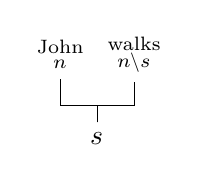
\begin{tikzpicture}
\tikzset{grow' = up}
\tikzset{frontier/.style={distance from root=30pt}}
\tikzset{edge from parent/.style=
{draw,
edge from parent path={(\tikzparentnode.north)
-- +(0,6pt)
-| (\tikzchildnode)}}}
\Tree [.$s$ $\substack{\text{John}\\n}$
$\substack{\text{walks}\\n\textbackslash s}$ ]
\end{tikzpicture}
\item 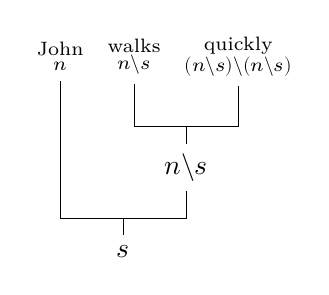
\begin{tikzpicture}
\tikzset{grow' = up}
\tikzset{frontier/.style={distance from root=70pt}}
\tikzset{edge from parent/.style=
{draw,
edge from parent path={(\tikzparentnode.north)
-- +(0,6pt)
-| (\tikzchildnode)}}}
\Tree [.$s$ $\substack{\text{John}\\n}$
[.$n\textbackslash s$
$\substack{\text{walks}\\n\textbackslash s}$
$\substack{\text{quickly}\\(n\textbackslash s)\textbackslash(n\textbackslash s)}$ ] ]
\end{tikzpicture}
\end{enumerate}


The above example is of a \textbf{undirectional grammar}. You can only work in one
direction, in the sense that if you have an expression of category
\(A\textbackslash B\), then you have to write an expression of type \(A\) on the
\emph{left-hand} side in order to obtain an expression of type \(B\). There are
many expressions which would result in a new expression if something were
written to their right. Take, for example, an adjective like \textbf{poor}. Together
with \textbf{John}, obtained from category \(n\), this gives us \textbf{poor John}. The
definition of derived categories can be modified in the following manner so
as to allow for expressions like this:
\begin{enumerate}
\setcounter{enumi}{4}
\item If \(A\) and \(B\) are categories, then both \((A\textbackslash B)\) and
\((A/B)\) are categories
\end{enumerate}


Thus we obtain a \textbf{bidirectional} categorial grammar. Such a categorial grammar
needs two syntactic rules:
\begin{enumerate}
\setcounter{enumi}{5}
\item \begin{enumerate}
\item If \(\alpha\) is in cateogry \(A\) and \(\beta\) is in cateogry \(A\textbackslash B\), then
\(\alpha\beta\) is in cateogry \(B\)
\item If \(\alpha\) is in category \(A/B\) and \(\beta\) is in category \(B\), then
\(\alpha\beta\) is in category \(A\)
\end{enumerate}
\end{enumerate}


In the example given in (16), both kinds of derived categories are involved
\begin{enumerate}
\setcounter{enumi}{15}
\item 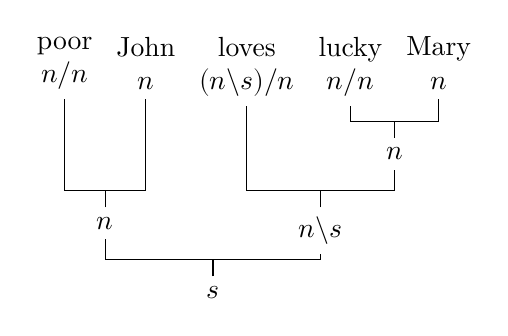
\begin{tikzpicture}
\tikzset{grow' = up}
\tikzset{frontier/.style={distance from root=90pt}}
\tikzset{level distance=25pt}
\tikzset{every tree node/.style={align=center,anchor=north}}
\tikzset{edge from parent/.style=
{draw,
edge from parent path={(\tikzparentnode.north)
-- +(0,6pt)
-| (\tikzchildnode)}}}
\Tree [.$s$
[.$n$ {poor\\$n/ n$} {John\\$n$} ]
[.$n\textbackslash s$ {loves\\$(n\textbackslash s)/n$}
[.$n$ {lucky\\$n/ n$} {Mary\\$n$} ] ] ]
\end{tikzpicture}
\end{enumerate}


In other variant of categorical grammar, expressions in derived categories
may be concatenated with several other expressions simultaneously.
\begin{enumerate}
\setcounter{enumi}{6}
\item If \(A,B,C\) are categories, then \(A\textbackslash B/C\) is a category
\item If \(\alpha\) is in cateogry \(A\), \(\beta\) is in category \(A\textbackslash B/C\), and
\(\gamma\) is in category \(C\), then \(\alpha\beta\gamma\) is in category \(B\)
\end{enumerate}


In this way, the transitive verb \textbf{loves} may be categories as
\(n\textbackslash s/n\), instead of as \((n\textbackslash s)/ n\)
\begin{enumerate}
\setcounter{enumi}{16}
\item 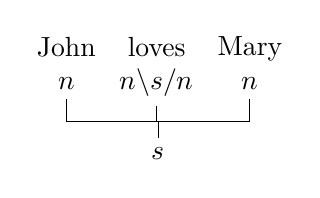
\begin{tikzpicture}
\tikzset{grow' = up}
\tikzset{frontier/.style={distance from root=40pt}}
\tikzset{level distance=25pt}
\tikzset{every tree node/.style={align=center,anchor=north}}
\tikzset{edge from parent/.style=
{draw,
edge from parent path={(\tikzparentnode.north)
-- +(0,6pt)
-| (\tikzchildnode)}}}
\Tree [.$s$ {John\\$n$} {loves\\$n\textbackslash s/n$}
{Mary\\$n$} ]
\end{tikzpicture}
\item 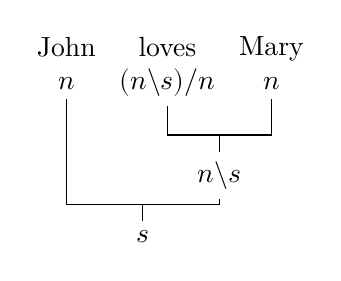
\begin{tikzpicture}
\tikzset{grow' = up}
\tikzset{frontier/.style={distance from root=70pt}}
\tikzset{level distance=25pt}
\tikzset{every tree node/.style={align=center,anchor=north}}
\tikzset{edge from parent/.style=
{draw,
edge from parent path={(\tikzparentnode.north)
-- +(0,6pt)
-| (\tikzchildnode)}}}
\Tree [.$s$ {John\\$n$}
[.$n\textbackslash s$ {loves\\$(n\textbackslash s)/n$}
{Mary\\$n$} ] ]
\end{tikzpicture}
\end{enumerate}


The analysis depicted in (17) attributes less structure to this example
sentence than the analysis in figure (18). In (18), \textbf{loves Mary} is treated as
a single constituent which is not so in (17). Generally speaking, an
analysis like that in (18) will be preferred. An exception is, for example,
formed by coordinative conjunctions, for which the categorization
\(s\textbackslash s/s\) is to be preferred over \(s\textbackslash(s/s)\) or
\((s\textbackslash s)/s\).
\begin{enumerate}
\setcounter{enumi}{18}
\item 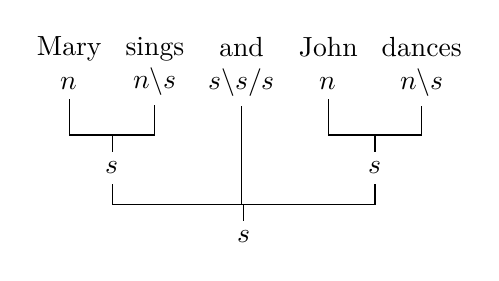
\begin{tikzpicture}
\tikzset{grow' = up}
\tikzset{frontier/.style={distance from root=70pt}}
\tikzset{level distance=25pt}
\tikzset{every tree node/.style={align=center,anchor=north}}
\tikzset{edge from parent/.style=
{draw,
edge from parent path={(\tikzparentnode.north)
-- +(0,6pt)
-| (\tikzchildnode)}}}
\Tree [.$s$
[.$s$ {Mary\\$n$} {sings\\$n\textbackslash s$} ]
{and\\$s\textbackslash s/s$}
[.$s$ {John\\$n$} {dances\\$n\textbackslash s $} ] ]
\end{tikzpicture}
\item 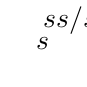
\begin{tikzpicture}
\tikzset{grow= up}
\tikzset{frontier/.style={distance from root=90pt}}
\tikzset{level distance=25pt}
\tikzset{every tree node/.style={align=center,anchor=north}}
\tikzset{edge from parent/.style=
{draw,
edge from parent path={(\tikzparentnode.north)
-- +(0,6pt)
-| (\tikzchildnode)}}}
\Tree [.$s$ ]
[.$s$
[.$s/ s$
[.$s$ {Mary\\$n$} {sings\\$n\textbackslash s$} ]
{and\\$s\textbackslash (s/s)$} ]
[.$s$ {John\\$n$} {dances\\$n\textbackslash s$} ] ]
\end{tikzpicture}
\end{enumerate}



The difference between a bidirectional categorial grammar and a context-free
grammar is in essence the following: A bidirectional categorial grammar
always indicates which of a given pair of constituents is dependent on the
other, whereas a context-free grammar need not always provide this information
\subsubsection{The Descriptive Adequacy of Categorial Grammar}
\label{sec:org2d471cf}
Compare sentences (22) and (23):
\begin{enumerate}
\setcounter{enumi}{21}
\item The job was quickly finished
\item The job was finished quickly
\end{enumerate}


In (22), the constituent \textbf{was finished} occurs discontinuously, that is, it is
interrupted by another expression. This contrasts with its continuity in
(23). In a categorial grammar in its pure form, this presents a problem.
Hence we are foreced to consider \textbf{was} and \textbf{finished} as separate lexical items
and to place each of them in (at least) two different cateogries, so they
can form both continuous and discontinuous constituents. Sentence (24) gives
another example of this phenomenon
\begin{enumerate}
\setcounter{enumi}{23}
\item John never calls up Mary, so she calls him up instead
\end{enumerate}


Here we have both a continuous and a discontinuous occurrence of the
constituent \textbf{calls up}. Here too, in a categorial grammar there is no choice
but to classify \textbf{calls up}, \textbf{calls} and \textbf{up} separately, as three distinct lexical items.

A second phenomenon which presents problems for pure categorial grammars and
context-free grammars centers around the intuition that sentence (25) means
the same as sentence (26):
\begin{enumerate}
\setcounter{enumi}{24}
\item John loves Mary, and Jack, Jill
\item John loves Mary, and Jack loves Jill
\end{enumerate}


(25) is derived from (26) by leaving out the word \textbf{loves} in the second
conjunct. Another conjecture is that the 'missing part' of (25) gets filled
in during the process of interpretation. Either way, leaving out a
constituent or filling one in introduces context-dependency into the
picture, since the piece to be left out or filled in must always be present
somewhere else in the structure.

A third phenomenon which illustrates that the limited generative capacity o
context-free grammars and pure categorial grammars may lead to unituitive
result is that of \textbf{word order}. Both kinds of grammar decree a fixed word
order and hence seem to fail as adequate descriptive tools for languages in
which it is not word order.
\subsubsection{Categorial Grammar and the Theory of Types}
\label{sec:org865b745}
\begin{enumerate}
\setcounter{enumi}{26}
\item 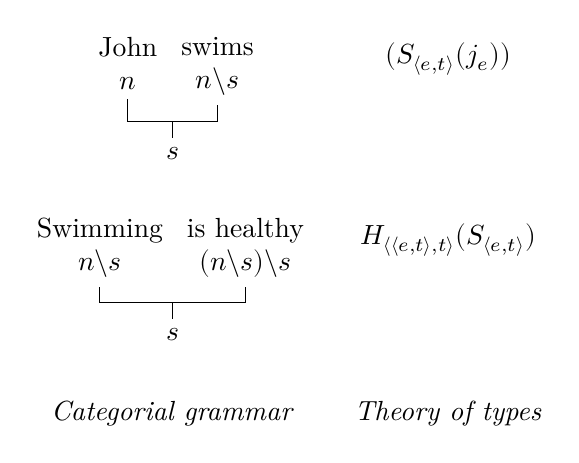
\begin{tikzpicture}
\tikzset{grow' = up}
\tikzset{frontier/.style={distance from root=40pt}}
\tikzset{level distance=25pt}
\tikzset{every tree node/.style={align=center,anchor=north}}
\tikzset{edge from parent/.style=
{draw,
edge from parent path={(\tikzparentnode.north)
-- +(0,6pt)
-| (\tikzchildnode)}}}
\Tree [.$s$ {John\\$n$}
{swims\\$n\textbackslash s$} ]
\begin{scope}[yshift=-2.3cm]
\Tree [.$s$ {Swimming\\$n\textbackslash s$}
{is healthy\\$(n\textbackslash s)\textbackslash s$} ]
\end{scope}
\begin{scope}
\node [xshift=3.5cm,yshift=1cm] {$(S_{\la e,t\ra}(j_e))$};
\node  [xshift= 3.5cm,yshift=-1.3cm] {$H_{\la\la e,t\ra,t\ra}(S_{\la e,t\ra})$};
\node [yshift=-3.5cm] {\textit{Categorial grammar}};
\node [yshift=-3.5cm,xshift=3.5cm] {\textit{Theory of types}};
\end{scope}
\end{tikzpicture}
\end{enumerate}
\subsection{\(λ\)-Abstraction}
\label{sec:org601423a}
\subsubsection{The \(λ\)-Operator}
\label{sec:orgf91a4ba}
\begin{enumerate}
\setcounter{enumi}{28}
\item Jogging is healthy
\end{enumerate}


A translation of this sentence into the theory of types may be obtained as
follows. Given that \textbf{jogging} expresses a property of individuals, the
expression may be translated as a predicate constant \(J\) of type \(\la
    e,t\ra\). \textbf{Healthy} expresses, a property of properties of individuals and is
as such to be rendered as a constant \(\calh\) of type \(\la\la e,t\ra,t\).
The whole of (29) is then to be translated as the formula \(\calh(J)\)

\begin{enumerate}
\setcounter{enumi}{29}
\item Not smoking is healthy
\item Drinking and driving is unwise
\item John admires John
\item John admires himself
\end{enumerate}


In order to account for constructions like these, the following rule is
added to the syntax of the theory of types as given in definition 2 in
\ref{def4.2.2}
\begin{enumerate}
\setcounter{enumi}{6}
\item If \(\alpha\) is expression of type \(a\) in \(L\), and \(v\) is a variable
of type \(b\), then \(\lambda v\alpha\) is expression of type \(\la b,a\ra\) in
\(L\)
\end{enumerate}


Let \(W\) be a constant of type \(\la e,t\ra\), and let \(x\) be a variable
of type \(e\). Then \(W(x)\) is a formula in which \(x\) appears as a free
variable. We can form the expression \(\lambda x(W(x))\) of type \(\la e,t\ra\).
We say that the expression \(\lambda x(W(x))\) has been formed from the expression
\(W(x)\) by \textbf{abstraction over} the free variable \(x\). We say that the free
occurrences of the variable \(x\) in \(\alpha\) are \textbf{bound} in \(\lambda x\alpha\) by the
\textbf{\(\lambda\)-operator} \(\lambda x\)

The interpretation of a \(\lambda\)-abstraction \(\lambda x_b\alpha_a\) is a
function. For this reason, \(\lambda\)-abstraction is also referred to as
\textbf{functional abstraction}.

Now we add the following clause to Definition 
\begin{enumerate}
\setcounter{enumi}{5}
\item If \(\alpha\in\WE^L_a\) and \(v\in\VAR_b\), then \(\llbracket \lambda
       v\alpha\rrbracket_{\bM,g}\) is that function \(h\in\bD_a^{\bD_b}\) s.t.
for all \(d\in\bD_b\):\(h(d)=\llbracket\alpha\rrbracket_{\bM,g[v/d]}\)
\end{enumerate}


Sentence (30), \emph{Not smoking is healthy}, can be translated as follows. Let
\(S\) be the translation of \emph{smoking}. This is a constant of type \(\la
    e,t\ra\). And let \(x\) be a variable of type \(x\). We obtain the
expression \(\lambda x\neg S(x)\) of type \(\la e,t\ra\). The whole of (30) may
now be obtained by applying the second-order predicate \(\calh\). The result
is \(\calh(\lambda x\neg S(x))\)
\subsubsection{\(λ\)-Conversion}
\label{sec:org30290b9}
The general notation for the result of replacing all free occurrences of a
variable \(v\) in an expression \(\beta\) by an expression \(\gamma\) is \([\gamma/v]\beta\)

\begin{definition}[]
A variable \(v'\) is \textbf{free for \(v\)}  in the expression \(\beta\) iff no free
occurrence of \(v\) in \(\beta\) is within the scope of a quantifier \(\exists v'\)
or \(\forall v'\) or a \(\lambda\)-operator \(\lambda v'\)
\end{definition}

\begin{theorem}[]
If all variables which occurs as free variables in \(\gamma\) are free for \(v\) in
\(\beta\), then \(\lambda v\beta(\gamma)\) and \([\gamma/v]\beta\) are equivalent
\end{theorem}
\subsubsection{The \(λ\)-Operator and Compositionality}
\label{sec:org57cc3cb}
The main purpose of translating a natural language into a formal language is
to obtain a semantic interpretation of the former via the semantics of the
latter. For the meaning of a correct translation is the same as the meaning
of what is translated. In order for the semantic interpretation to be
satisfactory, it is necessary that the process of translation comply to
certain requirements. Among these, two important requirements are that the
process be \textbf{explicit} and that it can be \textbf{specified in a finite manner}.  The
requirement that is be explicit means that it may not in any way rely on the
knowledge or creativity of the translator: it must be such that it could, at
least in principle, be automated. Furthermore, the translation process,
though essentially finite,must translate a potentially infinite number of
sentences.

One way of doing this is to stay closed to the syntactic rules of the
natural language in question, which are finite in number. Here we assume
that translations are available for all of the lexical elements of the
language, which are finite in number. The for each syntactic rule saying how
expressions may be combined to form composite expressions we formulate a
parallel rule, which says how the translations of these expressions may be
combined to give the translations of the composite expressions.

Now it should be clear that the way we have translated natural language
sentences into standard predicate logic up until now is neither explicit nor
compositional.
\begin{enumerate}
\setcounter{enumi}{34}
\item John smokes and drinks
\item \(Sj\wedge Dj\)
\end{enumerate}


The way of translating is not explicit, in that essential use is made of our
knowledge of the meaning of (35), in particular our knowledge of the fact
that (35) expressions a conjunction of two sentences. And it is not
compositional, in that no account is given of how the translation of (35) is
built up from the translations of \textbf{John} and \textbf{smokes and drinks}, or how the
translation of the \textbf{smokes and drinks} is built up from the translations of
\textbf{smokes} and \textbf{drinks}. Given that the lexical elements of (35) are rendered as
follows: \(John:j,smokes:S,drinks:D\), the phrase \textbf{smokes and drinks} can be
rendered as (37), while the whole of (35) translates as (38)
\begin{enumerate}
\setcounter{enumi}{36}
\item \(\lambda x(S(x)\wedge D(x))\)
\item \(\lambda x(S(x)\wedge D(x))(j)\)
\end{enumerate}


We shall introduce the first-order quantifiers \(\exists\) and \(\forall\)
categorematically by treating them as second-order predicates, that is to
say, as expressions of type \(\la\la e,t\ra,t\ra\)
\begin{center}
\(I(\exists)\) is that function \(f_{\exists}\in\{0,1\}^{(\{0,1\}^D)}\) s.t.
if \(h\in\{0,1\}^D\),then \par
\(f_\exists(h)=1\) iff there is a \(d\in D\) s.t. \(h(d)=1\) \par
\(I(\forall)\) is that function \(f_{\forall}\in\{0,1\}^{(\{0,1\}^D)}\) s.t.
if \(h\in\{0,1\}^D\),then \par
\(f_\exists(h)=1\) iff for all \(d\in D\) : \(h(d)=1\) 
\end{center}
In other words, \(I(\exists)\) is (the characteristic function of) the set
of non-empty subsets of, that is \(\{A\mid A\subseteq D\&A\neq\emptyset\}\).
And \(I(\forall)\) is (the characteristic function of) \(\{D\}\)

We have interpreted \(\exists\) as the set of all nonempty subsets of \(D\).
This means that the quantifier \(\exists\) is equivalent to the expression
\(\lambda Y\exists x(Y(x))\) in the theory of types.
\section{The Intensional Theory of Types}
\label{sec:org82111f2}
\subsection{Intensional Constructions and Intensional Concepts}
\label{sec:orgd778aa1}
Opaque contexts are also known as \textbf{intensional contexts}, and the expressions
and constructions they give rise to are likewise said to be intensional 

The intensionality of natural language is relevant at several different
points. To begin with, natural languages contain temporal, modal, and deontic
expressions, all of which involve intensionality. Besides these, it would
also need expressions which refer directly to intensional entities like
propositions, individual concepts and properties.
\begin{enumerate}
\item John asserts that the Dutch queen resides in the Hague
\end{enumerate}


Now the expression \textbf{assert} in (1) cannot stand for a relation between an
individual, in this case John, and a \textbf{sentence}, in this case
\begin{enumerate}
\setcounter{enumi}{1}
\item The Dutch queen resides in the Hague
\end{enumerate}


For (1) may well be true without John bearing any special relation to this or
any other English sentence. This suggests that \textbf{assert} is a relation, not
between individuals and sentences, but between individuals and \textbf{propositions}

If a logical theory is to provide representations of sentences which refer to
intensional entities like propositions, then it will need expressions which
stand for such entities.
\subsection{Syntax}
\label{sec:org26b40eb}
\begin{definition}[]
\(\bT\), the set of types in intensional type theory, is the smallest set
s.t.
\begin{enumerate}
\item \(e,t\in\bT\)
\item If \(a,b\in\bT\), then \(\la a,b\ra\in\bT\)
\item If \(a\in\bT\), then \(\la s,a\ra\in\bT\)
\end{enumerate}
\end{definition}

The vocabulary of any particular intensional, type-theoretical language \(L\)
consists once again of a part shared by all such languages, together with a
number of symbols which are peculiar to it. The shared part is
\begin{enumerate}
\item for every type \(a\), an infinite set \(\VAR_a\) of variables of type \(a\)
\item the connectives \(\wedge,\vee,\to,\neg,\leftrightarrow\)
\item the quantifiers \(\forall\) and \(\exists\)
\item the identity symbol =
\item the operators \(\Box,\Diamond,{}^\wedge,{}^\vee\)
\item the brackets ( and )
\end{enumerate}


The part which is peculiar to L consists of
\begin{enumerate}
\setcounter{enumi}{6}
\item for every type \(a\), a (possibly empty) set \(\CON_a^L\) of
constants of type \(a\)
\end{enumerate}


\begin{definition}[]
\begin{enumerate}
\item If \(\alpha\in\VAR_a\) or \(\alpha\in\CON_a^L\), then \(\alpha\in\WE_a^L\)
\item If \(\alpha\in\WE_{\la a,b\ra}^L\) and \(\beta\in\WE_a^L\), then \((\alpha(\beta))\in\WE_b^L\)
\item If \(\phi,\psi\in\WE_t^L\), then
\(\neg\phi,(\phi\wedge\psi),(\phi\vee\psi)\),\(\phi\to\psi\) and
\(\phi\leftrightarrow\psi\in\WE_t^l\)
\item If \(\phi\in\WE_t^L\) and \(v\in\VAR_a\), then \(\forall v\phi,\exists v\phi\in\WE_t^L\)
\item If \(\alpha,\beta\in\WE_a^L\), then \((\alpha=\beta)\in\WE_t^L\)
\item If \(\alpha\in\WE_a^L\) and \(v\in\VAR_b\), then \(\lambda v\alpha\in\VAR_{\la b,a\ra}\)
\item If \(\phi\in\WE_t^L\), then \(\Box\phi,\Diamond\phi\in\WE_t^L\)
\item If \(\alpha\in\WE_a^L\), then \({}^\wedge\alpha\in\WE_{\la s,a\ra}^L\)
\item If \(\alpha\in\WE_{\la s,a\ra}^L\), then \({}^\vee\alpha\in\WE_a^L\)
\item Every element of \(\WE_a^L\) for any \(a\) is constructed in a finite
number of steps using (1) - (9)
\end{enumerate}
\end{definition}

If \(\phi\in\WE_t^L\), then \({}^\wedge\phi\in\WE_{\la s,t\ra}^L\) refers to
the intension of \(\phi\), a function from possible worlds into truth values.
\subsection{Semantics}
\label{sec:orgf4efa98}
An expression of any intensional type \(\la s,a\ra\) is to be interpreted as
a function mapping possible worlds to elements of the interpretation domain
corresponding to type \(a\).

\begin{definition}[]
\begin{enumerate}
\item \(\bD_{e,D,W}=D\)
\item \(\bD_{t,D,W}=\{0,1\}\)
\item \(\bD_{\la a,b\ra,D,W}=\bD_{b,D,W}^{\bD_{a,D,W}}\)
\item \(\bD_{\la s,a\ra,D,W}=\bD_{a,D,W}^W\)
\end{enumerate}
\end{definition}

An expression of type \(\la s,t\ra\) thus refers to a function from possible
worlds to truth values. Functions of this kind will be called \textbf{propositions}.
An expression of type \(\la s,\la e,t\ra\ra\) refers to a function from
possible worlds to sets of individuals. Now sets of individuals serve as the
interpretations of predicates, and a predicate refers in different worlds to
different sets. This multiple reference of a predicate may be seen as a
function from possible worlds to sets of individuals, and this function may
be thought of as the predicate's intension. Any such intension will be called
a \textbf{property}

If \(\alpha\) is a constant of  type \(a\), then \(I(\alpha)\in\bD_a^W\). We refer to
\(\llbracket\alpha\rrbracket_{\bM,w,g}\) as the
\textbf{extension of \(\alpha\) in \(w\), given \(\bM\) and \(g\)}

\begin{definition}[]
\begin{enumerate}
\item If \(\alpha\in\CON_a^L\), then
\(\llbracket\alpha\rrbracket_{\bM,w,g}=I(\alpha)(w)\)

If \(\alpha\in\VAR_a\), then \(\llbracket\alpha\rrbracket_{\bM,w,g}=g(\alpha)\)

\item If \(\alpha\in\WE_{\la a,b\ra}^L\) and \(\beta\in\WE_a^L\), then
\(\llbracket\alpha(\beta)\rrbracket_{\bM,w,g}=\llbracket\alpha
       \rrbracket_{\bM,w,g}(\llbracket\beta\rrbracket_{\bM,w,g})\)

\item If \(\phi,\psi\in\WE_t^L\), then \(\llbracket\neg\phi\rrbracket_{\bM,w,g}=1\)
iff \(\llbracket\phi\rrbracket_{\bM,w,g}=0\)

\(\llbracket\phi\wedge\psi\rrbracket_{\bM,w,g}=1\) iff
\(\llbracket\phi\rrbracket_{\bM,w,g}=\llbracket\psi\rrbracket_{\bM,w,g}=1\)

\(\llbracket\phi\to\psi\rrbracket_{\bM,w,g}=0\) iff
\(\llbracket\phi\rrbracket_{\bM,w,g}=1\) and
\(\llbracket\psi\rrbracket_{\bM,w,g}=0\)

\(\llbracket\phi\leftrightarrow\psi\rrbracket_{\bM,w,g}\) iff
\(\llbracket\phi\rrbracket_{\bM,w,g}=\llbracket\psi\rrbracket_{\bM,w,g}\)

\item if \(\phi\in \WE_t^L,v\in \VAR_a\), then

\(\llbracket\forall v\phi\rrbracket_{\bM,w,g}=1\) iff for all
\(d\in\bD_{a,D}\):
\(\llbracket\phi\rrbracket_{\bM,w,g[v/d]}=1\)

\(\llbracket\exists v\phi\rrbracket_{\bM,w,g}=1\) iff there is at least one
\(d\in\bD_{a,D}\) s.t.: \(\llbracket\phi\rrbracket_{\bM,w,g[v/d]}=1\)

\item If \(\alpha,\beta\in \WE_a^L\), then
\(\llbracket\alpha=\beta\rrbracket_{\bM,w,g}=1\) iff
\(\llbracket\alpha\rrbracket_{\bM,w,g}=\llbracket\beta\rrbracket_{\bM,w,g}\)

\item If \(\alpha\in\WE_a^L\) and \(v\in\VAR_b\), then \(\llbracket\lambda
      v\alpha\rrbracket_{\bM,w,g}\) is that function \(f\in\bD_a^{\bD_b}\) s.t.
for all \(d\in \bD_b\):\(h(d)=\llbracket\alpha\rrbracket_{\bM,w,g[v/d]}\)

\item If \(\phi\in\WE_t^L\), then

\(\llbracket\Box\phi\rrbracket_{\bM,w,g}=1\) iff for all \(w'\in W\):
\(\llbracket\phi\rrbracket_{\bM,w',g}=1\)

\(\llbracket\Diamond\phi\rrbracket_{\bM,w,g}=1\) iff for some \(w'\in W\):
\(\llbracket\phi\rrbracket_{\bM,w',g}=1\)

\item If \(\alpha\in\WE_a^L\), then
\(\llbracket{}^\wedge\alpha\rrbracket_{\bM,w,g}\) is that function
\(h\in\bD^w_a\) s.t. for all \(w'\in W\): \(h(w')=\llbracket\alpha\rrbracket_{\bM,w',g}\)

\item If \(\alpha\in\WE^L_{\la s,a\ra}\), then
\(\llbracket{}^\vee\alpha\rrbracket_{\bM,w,g}=
      \llbracket\alpha\rrbracket_{\bM,w,g}(w)\)
\end{enumerate}
\end{definition}

\begin{definition}[]
If \(\alpha\in\WE_a^L\), then \(\Int_{\bM,g}(\alpha)\) is that \(h\in\bD^W_a\)
s.t. for all \(w'\in W\):\(h(w')=\llbracket\alpha\rrbracket_{\bM,w',g}\)
\end{definition}
\end{document}
